\chapter{Large Sphere Experiment} %new name?
\label{chap:LargeSphere}

\textit{The work presented here has been presented previously as an oral presentation at AIC 2013 \citep[p. 623]{macdonald_chromatic_2013} \textbf{prior to the author's involvement}, and as an oral presentation at ICVS 2017 \citep[p. 35/58]{jan_kremers_24th_2017} by the author.}

\section{Summary}

The goal of this experimental work was to examine the effect of different wavelengths of light upon chromatic adaptation. Our hypothesis was that \gls{ipRGC} stimulation may need to be considered in order to fully model the induced adaptation, with the null hypothesis being that chromatic adaptation can be fully accounted for by cone and rod mechanisms.

Within a Ganzfeld viewing environment, illuminated by one of 16 different wavelengths of near-monochromatic light, observers performed an achromatic setting task, controlling the chromaticity of a display visible in the central field through a 4$^{\circ}$ circular aperture with two handheld sliders.

Code and data??????? %%%%%

Results:

This project was designed before the author arrived at \gls{UCL}, and data from two participants had already been collected. Data collection required at least 16 hours commitment from observers, and so the only observers up to that point had been LM (one of the authors academic supervisors), who initiated the experiment, and TR who \dots %%%
The original goal for my involvement in this project was that I should be a third observer, and assist in the data analysis. However, following the collection and initial data analysis of my own data, it became clear that there had been a technical fault during this run of data collection, and my data was deemed corrupted. This data is discussed further in Appendix X. %%%%%%%%
Thus, my only contribution to this work is an extension to the data analysis started by LM, upon which I shall focus on in this chapter.

\section{Methodology}

\subsection{Hardware}

A hollow fibreglass sphere of approximately 750mm diameter was prepared with three holes; the first for an observer's face, the second (above) for an illuminant to illuminate the Ganzfed, and the third (opposite the first) through which a small portion of an LCD screen could be seen. The interior of the sphere was painted with RAL 7040 dulux vinyl matt, of approximately 38\% reflectance. Illumination was provided by a Kodak slide projector, filtered through one of 16 near-monochromatic filters, ranging in 20nm intervals from 400-700nm inclusive. % Add something about `mesopic'

\begin{figure}[htbp]
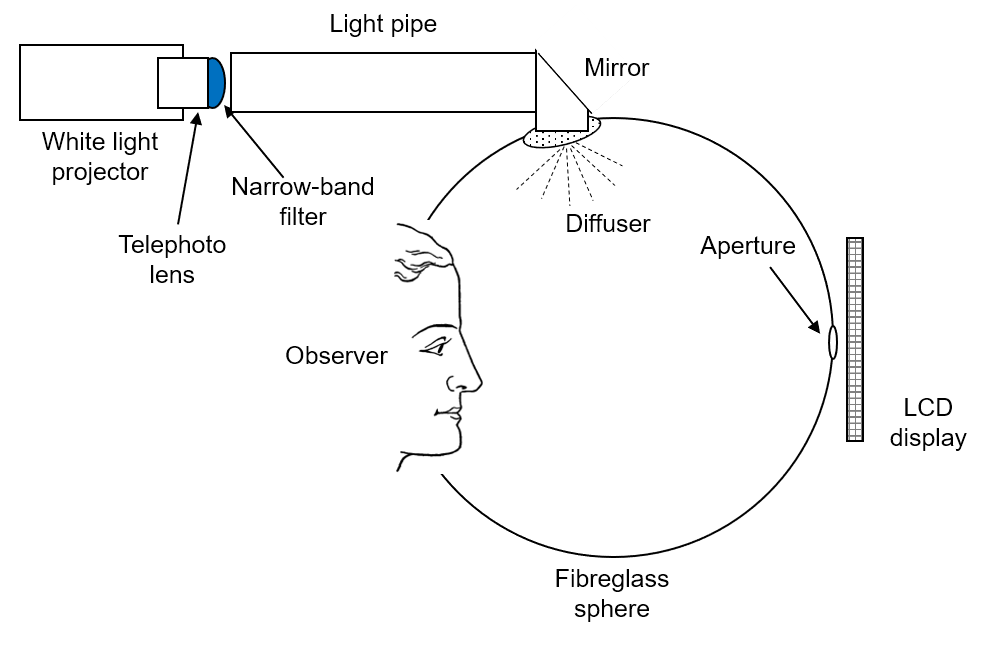
\includegraphics[max width=\textwidth]{figs/LargeSphere/sketch.png}
\caption{The hardware design. Illustration courtesy of Lindsay MacDonald.}
\label{fig:sketch}
\end{figure}

\begin{figure}[htbp]
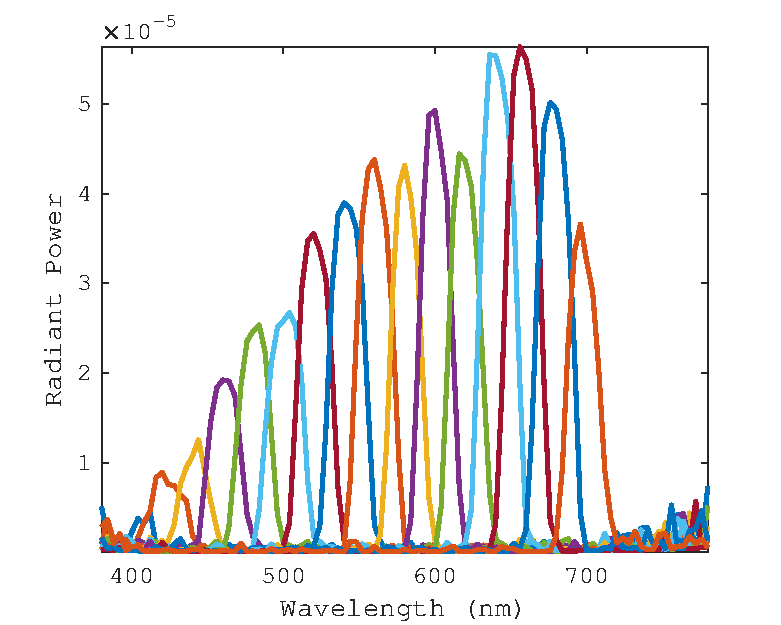
\includegraphics[max width=\textwidth]{figs/LargeSphere/LSillum.pdf}
\caption{The illuminants within the sphere, created by filtering light from a slide projector, measured as reflecting from a point just to the right of the aperture through which an observer would view the screen. Measurements made by Lindsay MacDonald.} %%%%%%?????
\label{fig:LSillum}
\end{figure}

\subsection{Observer task}

The observer sat on one side of the sphere with their face inside the sphere, such that nothing outside of the sphere was visible. On view on the opposite side of the sphere was a circular 4$^{\circ}$ aperture onto an LCD screen, upon which a random colour drawn from ??????%
was visible. It was the observer's task to use two handheld sliders, which controlled the chromaticity of the screen, to make the appearance of the screen achromatic. Once they were happy with the achromacy of the patch, they were to hit a button at which a new random colour would be presented. The first displayed colour was displayed at L* of 85, with subsequent colours descending by 5 L* until 15 L*. This scale was repeated 10 times per session. Per session observers made 10 selections at 16 lightness levels (160 total). Observers performed 16 sessions (2560 selections total). See Figure \ref{fig:ExperimentalPro}.

\begin{figure}[htbp]
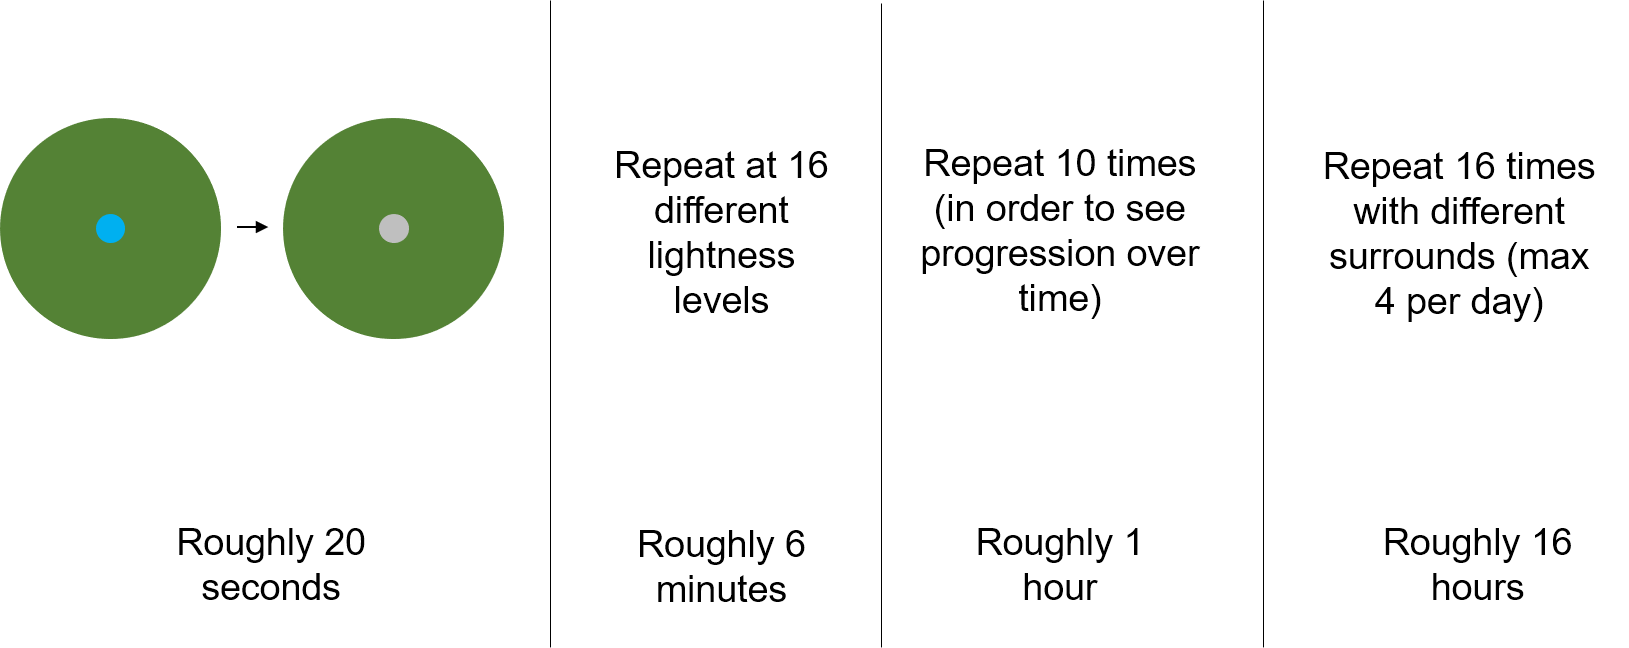
\includegraphics[max width=\textwidth]{figs/LargeSphere/ExperimentalPro.png}
\caption{The experimental protocol.}
\label{fig:ExperimentalPro}
\end{figure}

\subsection{Data Collection}

Data was collected for two observers \dots

\subsection{Data Processing}

Two distinct approaches were taken to data processing. The first attempted to process the data in a chromatic space, with the reasoning that under the null condition chromatic selections should simply correspond to the chromaticity of the surround illuminants. If it were shown that this relationship was not as expected, in a manner which might suggest involvement by other mechanisms (meaning rods or \glspl{ipRGC}), then this could be considered as evidence against the null hypothesis.

The second approach took advantage of the fact that measurements were taken at samples across the wavelength spectrum. Here the logic was that if the null condition were true, we should be able to fit a model to observer responses which only used cone-based inputs, and we could carefully consider the (presumed) benefit of including rods and \glspl{ipRGC} in the model. If either rod input or \gls{ipRGC} input were found to dramatically improve the model then this could be considered as evidence against the null hypothesis.

\section{Results}

\subsection{Chromaticity-based analysis}

\hl{As presented at ICVS.}

\subsection{Spectrum-based analysis}

Code: (?) %%

The first stage of this analysis was to generate simulated data which represented the situation whereby there was only simple Von Kries adaptation. This was accomplished by multiplying the individual \glspl{SPD} (Figure \ref{fig:LSillum}) by the CIE 2006 10$^{\circ}$ observer fundamentals (not in the manner in which this is usually done, resulting in tristimulus values, but rather poitwise, thus retaining the spectral nature of the data). See Figure \ref{fig:LSsimdata}.

\begin{figure}[htbp]
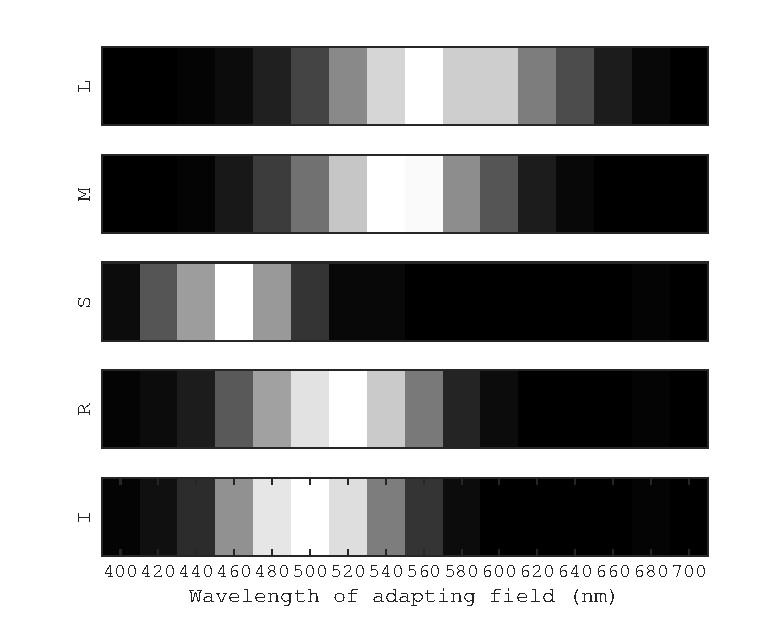
\includegraphics[max width=\textwidth]{figs/LargeSphere/LSsimdata.pdf}
\caption{Simulated data for a basic Von Kries observer. In this figure white represents a high response. For example, with 560nm peripheral stimulation we would expect an observer to pick a colour with high L-cone activation as achromatic, assuming that the sensitivity of L-cones had been suppressed and thus higher activation was required to reach a neutral point (see peak roughly in the centre of the top bar).}
\label{fig:LSsimdata}
\end{figure}

A comparison was then made between this data and a set of real data (Obs = TR, averaged over time (entire run, no exclusions), averaged over L* = 35:60\footnote{Values outside of this range exhibited gamut boundary issues.}). This real data had been transformed from the recorded RGB values of achromatic matches into LMS values. It can be seen that there is a considerable difference between the simulated data and the real data (Figure \ref{fig:simVreal}). S-cone data shows the closest match, with the predicted peak at 460nm\footnote{Note that this is not at the peak sensitivity of s-cones (which would appear at 440nm for this dataset at 20nm intervals) but rather at the peak of the s-cone sensitivity function multiplied by the \gls{SPD}, as plotted in Figure \ref{fig:LSsimdata}.} being mirrored in the real data. This peak appears to bleed into the (real) M-cone data, and the simulated data for L and M-cone data shows very little correspondence to the collected data. Correlation coefficients between the simulated and this specific real dataset are 0.1399, -0.2509, 0.3164 for L, M and S respectively.

\begin{figure}[htbp]
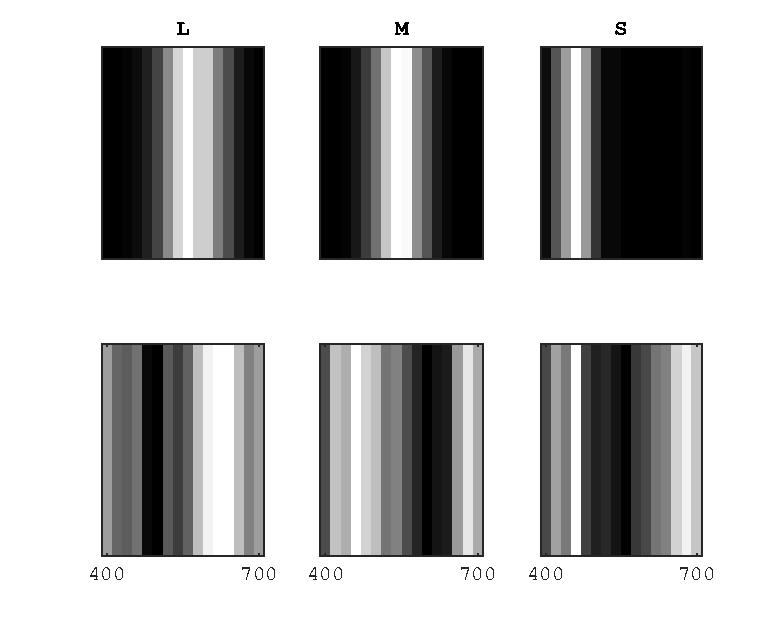
\includegraphics[max width=\textwidth]{figs/LargeSphere/simVreal.pdf}
\caption{A comparison of simulated data (top row) and real data (bottom row). Data from the top row is as per the top three bars of Figure \ref{fig:LSsimdata}.}
\label{fig:simVreal}
\end{figure}

In order to understand the way in which adaptation may be crossing between channels, or the way in which we may have not properly isolated our channels (it is unclear exactly how much freedom an observer truly has to move around the response space) a brute-force method was used to find combinations of the above simulated data which would best fit the real data.

10000 random sets of weighting values (30000 values total) between -25 and 25\footnote{An analysis showed that the absolute range of these figures was unimportant, since we were looking for correlation with the real data rather than absolute correspondence. Thus they are listed here only to assist the reader in understanding graphs such as Figure \ref{fig:contributions_3}.} were generated. These weightings were applied to the simulated responses and the results were additively combined\footnote{(X amount of simulated L) + (Y amount of simulated M) + (Z amount of simulated S)}. The correlation between this new random combination and each channel of the real data was computed. The top performing randomly generated combinations were selected and are presented in Figure \ref{fig:maxsimVreal}. These particular combinations were created through cross-combining the original simulated data (top row of Figure \ref{fig:simVreal}), in the ratios shown in Table \ref{tab:crosscomb} and correlated with the real data to extent of the following coefficients: 0.9126, 0.8861, and 0.7726 for L, M and S respectively. These are much improved over the coefficients for the original simulated data.


\begin{table}[hbtp]
\centering
\begin{tabular}{|r|r|r|r|}
\hline
 & L & M & S \\ \hline
L & $18.4069$ & $-23.2578$ & $-10.9817$ \\ \hline
M & $-13.0477$ & $9.8327$ & $10.6844$ \\ \hline
S & $-2.7633$ & $-17.6798$ & $8.3036$ \\ \hline
\end{tabular} % Would be nice to format to fit page width
\caption{Optimal weights to fit the specific real dataset used. \\ \emph{Example: Image in top left of Figure \ref{fig:maxsimVreal} (L) was created by combining 18.4069 * the original simulated L (Top left of Figure \ref{fig:simVreal}), -23.2578 * the original simulated M and -10.9817 * the original simulated S.}}
\label{tab:crosscomb}
\end{table}

\begin{figure}[htbp]
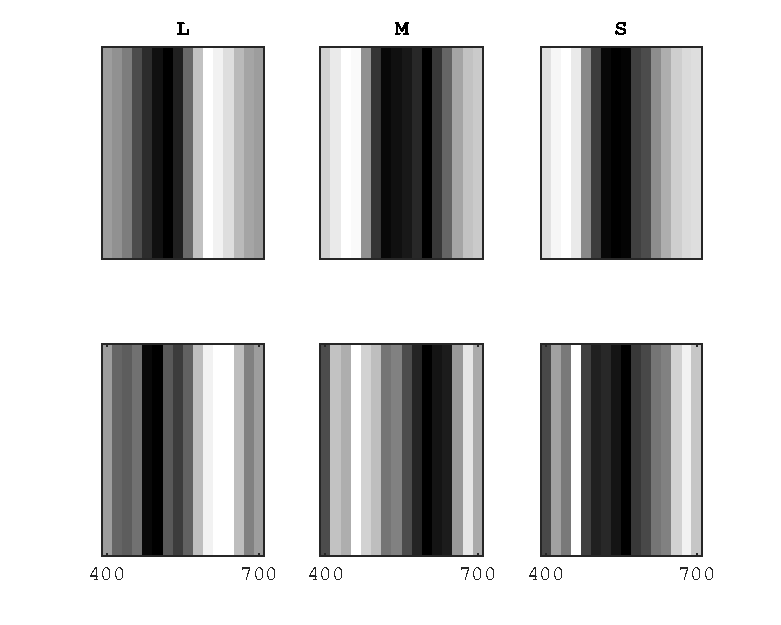
\includegraphics[max width=\textwidth]{figs/LargeSphere/maxsimVreal.pdf}
\caption{A comparison of randomly generated combinations (top row) whereby channels were freely mixed from basic Von Kries simulated data (top row of Figure \ref{fig:simVreal}) to best correlate with real data, and real data (bottom row) (repeated from Figure \ref{fig:simVreal}).}
\label{fig:maxsimVreal}
\end{figure}

\begin{figure}[htbp]
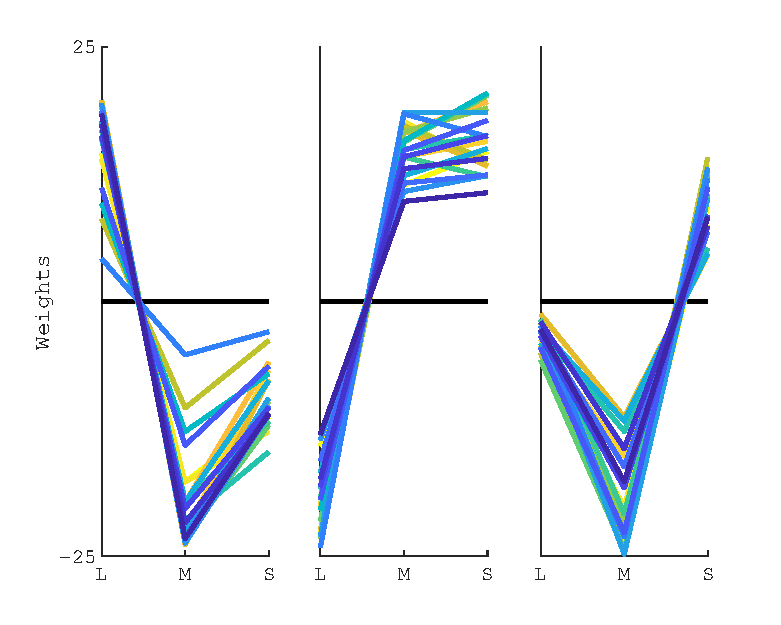
\includegraphics[max width=\textwidth]{figs/LargeSphere/contributions_3.pdf}
\caption{Top 0.2\% performing randomly generated combinations, presented in terms of the weights of the original simulated data that they use. The subfigure on the left represents the weights needed to reconstruct the real data for L, the middle - M, and the right - S. Colour coded such that dark blue is the highest performing and yellow is the worst performing (of this highly performing subset).}
\label{fig:contributions_3}
\end{figure}

\begin{figure}[htbp]
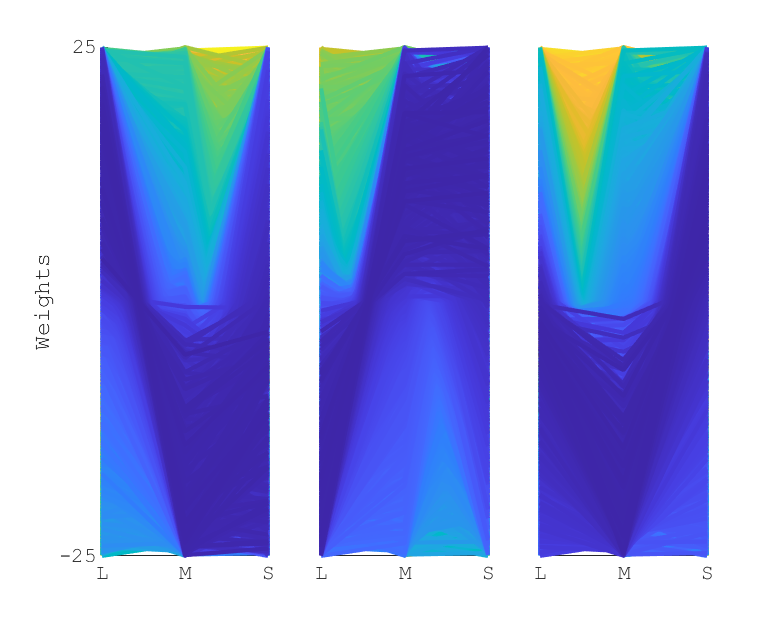
\includegraphics[max width=\textwidth]{figs/LargeSphere/contributions_all.pdf}
\caption{As per Figure \ref{fig:contributions_3} but for all randomly generated combinations. The trends seen in Figure \ref{fig:contributions_3} are visible, and the range of these trends (extending into the poorer performing randomly generated combinations) can be seen. The colours are rescaled such that yellow now represents the worst performing randomly generated combinations of the entire set. Plots are plotted ordered by success and so lines representing successful randomly generated combinations will overlay lines representing poorer performing ones.}
\label{fig:contributions_all}
\end{figure}

The top performing 0.2\% of the randomly generated combinations are presented in terms of their components (analogous to plotting the values in \ref{tab:crosscomb}) in Figure \ref{fig:contributions_3}, and the entirety of the results for the randomised sampling presented in Figure \ref{fig:contributions_all}. 

It can be seen that to reconstruct the real data for L, a high amount of simulated L, and a low amount of both simulated M and S are required, though from Figure \ref{fig:contributions_all} it can be seen that the requirement for low S is less stringent. It can also be seen that the amount of L required seems related to the amount of M required (from the way in which the lines cross at a point).

A similar but opposite trend is visible for M.

For S, there is a narrow range of successful values for L (negative but close to 0), a larger range of strongly negative values for M, and a range of positive values for S. The reciprocal relationship between L and M seen in the reconstructions of L and M is no longer visible, but instead there is a new reciprocal relationship visible between M and S, though examination of Figure \ref{fig:contributions_all} suggests that this is not as important as in the case of L and M.

It is reassuring that in each case, successful random combinations used high positive levels of the target signal. For both L and S the target signal was the only positive weighting, with M taking positive weights of both M and S. 

\subsubsection{Adding rods and ipRGCs}

In order to investigate whether rods or \glspl{ipRGC} were playing a role in adaptation as measured by this dataset, the analysis was re-run with the additional rod input, additional \gls{ipRGC} input, and both rods and \glspl{ipRGC} as additional inputs. See Figure \ref{fig:LSsimdata} for a visualisation of these channels. The results of re-running the computations following the addition of these inputs is shown in Table \ref{tab:plusres}. Minor increases in correlation are exhibited. However, it should be noted that one would expect to see at least a minor increase in ability from practically any additional signal, so long as it differed from the already accessible signals.

\begin{table}[hbtp]
\centering
\begin{tabular}{|r|r|r|r|}
\hline
Just cones: & $0.9126$ & $0.8861$ & $0.7726$ \\ \hline
+ rods: & $0.9156$ & $0.8881$ & $0.7987$ \\ \hline
+ ipRGCs: & $0.9218$ & $0.8867$ & $0.8055$ \\ \hline
+ rods + ipRGCs: & $0.9326$ & $0.8933$ &$0.8100$ \\ \hline
\end{tabular} % Would be nice to format to fit page width
\caption{Correlation coefficients for various conditions incorporating additional signals.}
\label{tab:plusres}
\end{table}

Further, it is not clear to what extent the gains exhibited in Table \ref{tab:plusres} are due to noise within the computations; the randomly generated combinations are set via a random number generator which is re-set each time the script is run for reproducibility, however there is nothing to stop the randomly generated values for the additional input runs performing better purely by chance alone. In order to investigate this, the above extensions were re-run 100 times each, and the top performance for each skimmed and saved. The results of this are presented in Figure \ref{fig:relcontributions}. From this figure it can be seen that there is a real and clear benefit from the inclusion of the additional signals, and from inclusion of \emph{both} of the additional signals.

\begin{figure}[htbp]
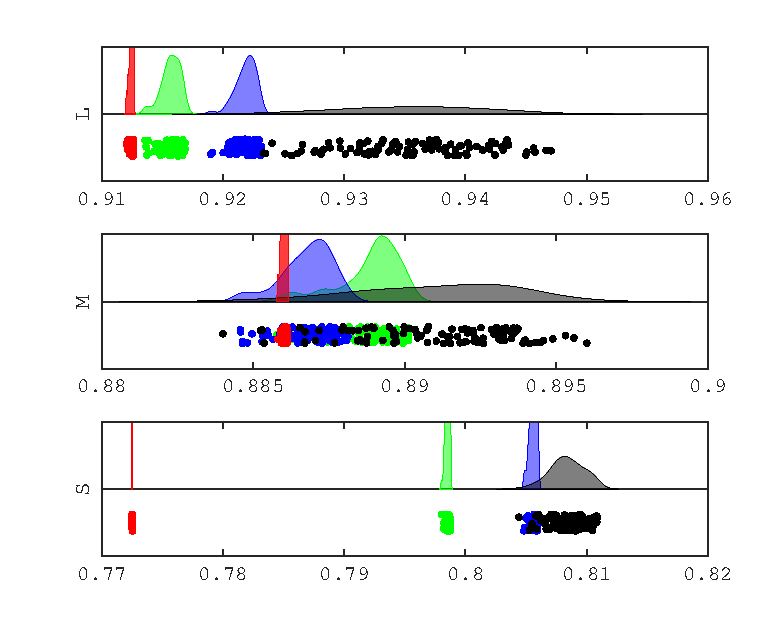
\includegraphics[max width=\textwidth]{figs/LargeSphere/relcontributions.pdf}
\caption{Raincloud plot \cite{allen_raincloud_2019} showing the results of re-running the extended analyses 100 times and skimming the best performer from each. Red points and probability density function represent `just cones', green - `+ rods', blue - `+ \glspl{ipRGC}', black - `+ rods + \glspl{ipRGC}'.}
\label{fig:relcontributions}
\end{figure}

\section{Discussion}

There is a clear distinction between the simple simulated response functions, and the recorded data. It is interesting that a simple linear recombination can improve the correlation so greatly. It should be remembered however that this type of post-hoc fitting is liable to delivering the results a researcher might hope to find. 

Taken at face value, the results seem to indicate that the principal drivers of adaptation are not at the cone level, but rather at a higher level, once cone inputs have been combined. The results mirror what might be expected of these higher level signals - there appears to be a single signal for L and M, roughly mirrored between the two, with a reciprocal trade-off possible between L and M for both, and the S cone signal takes positive weights for S, and negative weights for both L and M, but with a curious hint of a reciprocal trade-off between S and M.

However, it is unclear to what extent these relationships may arise due to limitations of the experimental set-up; it is possible that a rise in one signal is yoked through hardware limitation to the rise or fall in another. Future investigators should consider whether this effect is modellable.

\subsection{Additional Signals}

Though there is a demonstrated ability of additional signals to improve the correlation with the real data, it would be a considerable leap to consider this as evidence for the existence of mechanisms operating in this manner.

It is likely that any additional signal at a different wavelength (or even with a different frequency component) would have been able to deliver a higher correlation, since the data is noisy and through the random recombination we are functionally allowing every option to be tested. This is highly likely to result in over-fitting. One way to test whether this has occurred is to plot the contributions of the top performers from these situations (analogous to Figures \ref{fig:contributions_3} and \ref{fig:contributions_all}) and consider whether there are any trends. If the improvements are meaningful (rather than simply fitting to noise) we would be more likely to see trends in the optimal weightings. This is plotted in Figure \ref{fig:contributions_5}. It can be seen that there does appear to be some trends for both rods and \glspl{ipRGC}. Splitting this apart, into Figures \ref{fig:contributions_4} and \ref{fig:contributions_5minusrods}, where we plot the results for simulations run where only the rods were added or only the \glspl{ipRGC} were added, we can see these trends slightly more clearly.

\begin{figure}[htbp]
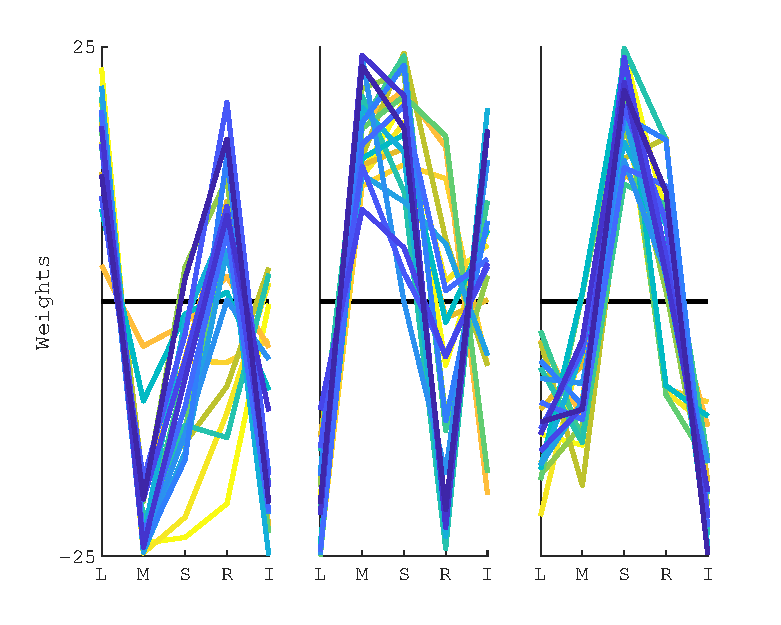
\includegraphics[max width=\textwidth]{figs/LargeSphere/contributions_5.pdf}
\caption{As per Figure \ref{fig:contributions_3} but for the conditions where both rods and ipRGCs were included as additional input signals were considered.} 
\label{fig:contributions_5}
\end{figure}

\begin{figure}[htbp]
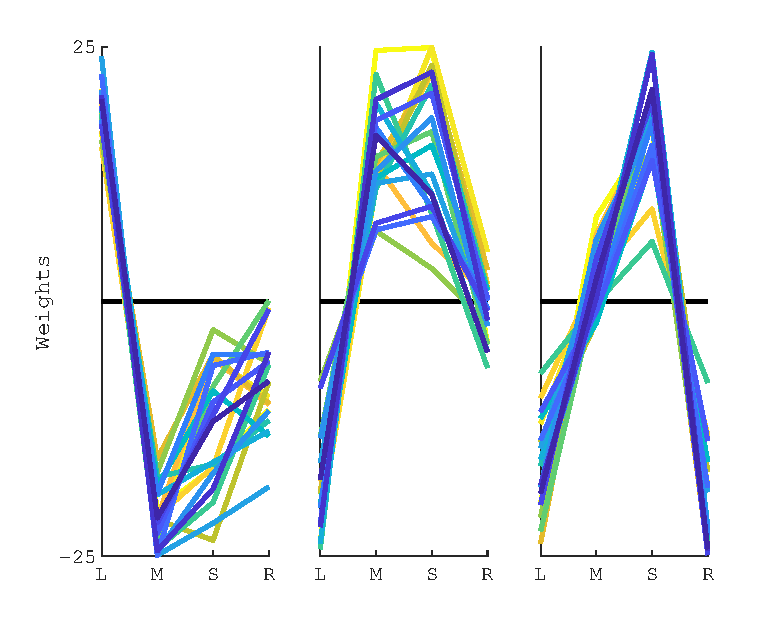
\includegraphics[max width=\textwidth]{figs/LargeSphere/contributions_4.pdf}
\caption{As per Figure \ref{fig:contributions_3} but for the conditions where rods were included as additional input signals.} 
\label{fig:contributions_4}
\end{figure}

\begin{figure}[htbp]
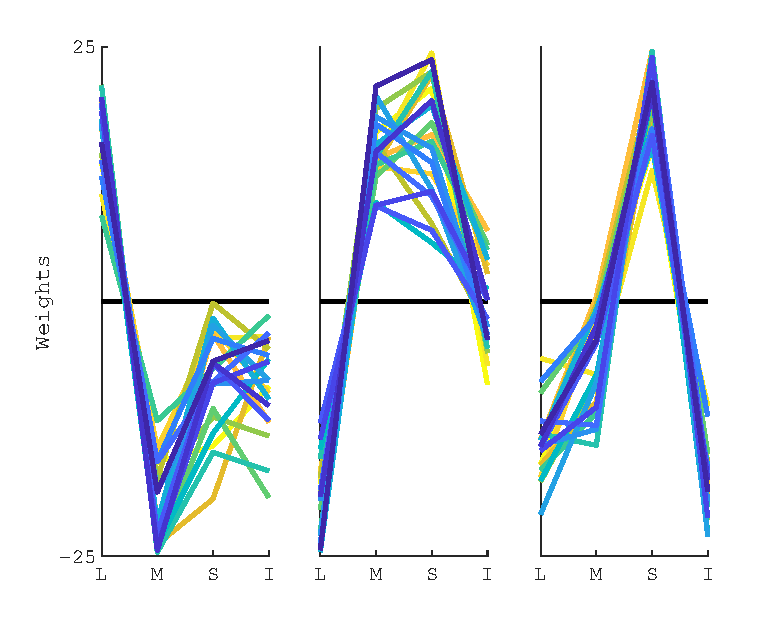
\includegraphics[max width=\textwidth]{figs/LargeSphere/contributions_5minusrods.pdf}
\caption{As per Figure \ref{fig:contributions_3} but for the conditions where ipRGCs were included as additional input signals.} 
\label{fig:contributions_5minusrods}
\end{figure}

Figures \ref{fig:contributions_4} and \ref{fig:contributions_5minusrods} appear somewhat similar. Considering the similar spectral characteristics of rods and melanopsin, it should be expected that the model would use the signals in somewhat similar fashions. It appears as though neither have a particularly strong role to play in the L and M adaptation, however both seem to reliably be used as a negative weighting for S. It is unclear whether this is simply a response to a single high datapoint in this dataset (the peak at 460nm) or whether this integration serves a broader purpose. This peak at 460nm also seems to be the cause for the stubbornly low correlation coefficients for the S channel (compared to L and M), which max out at around 0.81 (see Figure \ref{fig:relcontributions}). 

\section{Conclusion}












There are a number of possibilities for why this is not possible; non-linear, other mechanisms, noise (there is reason to believe that the data should be highly self-correlated over a single session but less so between sessions/conditions)



%Simplifications were made to consider only an average L* value (between and one timepoint 



Further investigations might add time dependency

Try the other datasets we have //
\dots possibly with more precise observer models for each.

I'd also like to try having a different observer for central and peripheral.

Consider different time points.	

Trichromatic display - 
It is unclear what the nature of the display, regards limiting the ability of the respondant to freely 

% Strong self correlation. Unsure whether the results are because of self correlation or because of genuine responses (sharpened cone spectra?)


This is a minimal improvement. Therefore, I do not reject the null hypothesis in this case.
